\chapter{Architecture}
\section{OMNI Compiler}
The \clawfcomp is based on the \omni\cite{omni:website}. The \omni Project
provides a set of programs to build source-to-source translator for C/C++
and FORTRAN. It is jointly developed by the Programming Environment Research
Team of the RIKEN AICS and the HPCS Lab. of the University of Tsukuba both
located in Japan. In the case of the \clawfcomp, we are using only the FORTRAN
capabilities of the \omni. The FORTRAN front-end and back-end are still
actively developed as of today and contribution can be made on their master
repository\cite{omni:github}.

\subsection{The FORTRAN front-end}
The FORTRAN front-end is the program that parses FORTRAN source code and that
generates the \gls{ir}. Its grammar is written in \lstinline|yacc| and the
processing and \gls{ir} generation is written in \lstinline|C|. This program
can be called individually as shown in listing \ref{lst:ffront}.

\begin{lstlisting}[label=lst:ffront, language=Bash, caption=Call F\_Front]
F_Front -M my_module_dir -o my_program.xml my_program.f90
\end{lstlisting}

As the \omni acts as a compiler, it also has a notion of module. When a FORTRAN
module is parsed with the front-end, a \lstinline|.xmod| file is generated.
This file contains all the signatures included in the module. This file is then
needed to parse other FORTRAN code depending on the module.

\begin{lstlisting}[label=lst:m1, language=Fortran, caption=module\_m1.f90]
MODULE m1
  USE m2
END MODULE m1
\end{lstlisting}

\begin{lstlisting}[label=lst:m2, language=Fortran, caption=module\_m2.f90]
MODULE m2
  USE m3
END MODULE m2
\end{lstlisting}

\begin{lstlisting}[label=lst:m3, language=Fortran, caption=module\_m3.f90]
MODULE m3
END MODULE m3
\end{lstlisting}

If we take the simple example shown in listings \ref{lst:m1}, \ref{lst:m2} and
\ref{lst:m3}, where we have a module 1 depending on module 2 and module 2
depending on module 3. These source files should be processed by the front-end
as shown in listing \ref{lst:ffrontdep}.

\begin{lstlisting}[label=lst:ffrontdep, language=Bash, caption=Parse module with dependencies]
F_Front -o module_m3.xml module_m3.f90      # produces m3.xmod
F_Front -M . -o module_m2.xml module_m2.f90 # uses m3.xmod and produces m2.xmod
F_Front -M . -o module_m1.xml module_m1.f90 # uses m2.xmod and produces m1.xmod
\end{lstlisting}


\subsection{\xcodeml}
\xcodeml\cite{omni:xcodemlf95,omni:xcodemlf2008} is the \gls{ir} used by the
translator in the CLAW FORTRAN Compiler. This \gls{ir} is based on the XML
format and is described in a specification document. It allows to have an
high-level representation of FORTRAN 2008 programs.

Listing \ref{fortran1} is a simple FORTRAN program. Its \xcodeml \gls{ir} is
shown in listing \ref{xcodeml1}. A typical \xcodeml translation unit is
composed of the followings sections:
\begin{itemize}
\item Type table with all the type definitions used in the translation unit
(Listing \ref{xcodeml1} line 6-24).
\item Global symbols table listing all the symbols at global scope (Listing
\ref{xcodeml1} line 25-29).
\item Global declarations section listing the actual function and/or module
declarations (Listing \ref{xcodeml1} line 30-82).
\end{itemize}

\lstinputlisting
  [
    label=fortran1,
    caption=Basic FORTRAN program,
    language=Fortran
  ]{code/basic_fortran.f90}

\lstinputlisting
  [
    label=xcodeml1,
    caption=\xcodeml IR,
    language=xml
  ]{code/basic_fortran.xml}

\subsection{The FORTRAN back-end}
The FORTRAN back-end is the program that decompiles \gls{ir} back to FORTRAN
code. It is a simple Java program that implements a visitor patterns across
the \gls{ast}. It can be called as a standalone program or directly within the
translator as it is done in the \clawfcomp.

\section{\clawfcomp}

The \clawfc is the program handed to the end-user. It performs all the needed
step to have a source-to-source translation of a FORTRAN program. As shown in
Figure \ref{fig:clawfc_main_workflow}, it is composed by various programs
under-the-hood. The complete workflow is devided as follows:

\begin{enumerate}
\item \textbf{FPP}: The FORTRAN source code is preprocessed by a standard
FORTRAN preprocessor. Typically the one provided by the default compiler.
The \lstinline|FC| environment variable is used by the CMake build system to
determine it.
\item \textbf{F\_Front}: The preprocessed FORTRAN source code is then parsed
by the OMNI Compiler FORTRAN Front-end to produce the input \xcodeml \gls{ir}.
\item \textbf{CX2X}: The input \xcodeml \gls{ir} is manipulated according to
the rules of the CLAW directive language. It produces the output \xcodeml
\gls{ir}.
\item \textbf{F\_Back}: The output \xcodeml \gls{ir} is analyzed to produce
the transformed FORTRAN code.
\end{enumerate}

\ffront{}, \fback{} are part of the \omni{}, \fpp{} is provided by the
installed FORTRAN compiler. The \xcodeml to \xcodeml translator \cx2x{} is
actively developed as part of the CLAW project.

\begin{figure}[!ht]
  \centering
  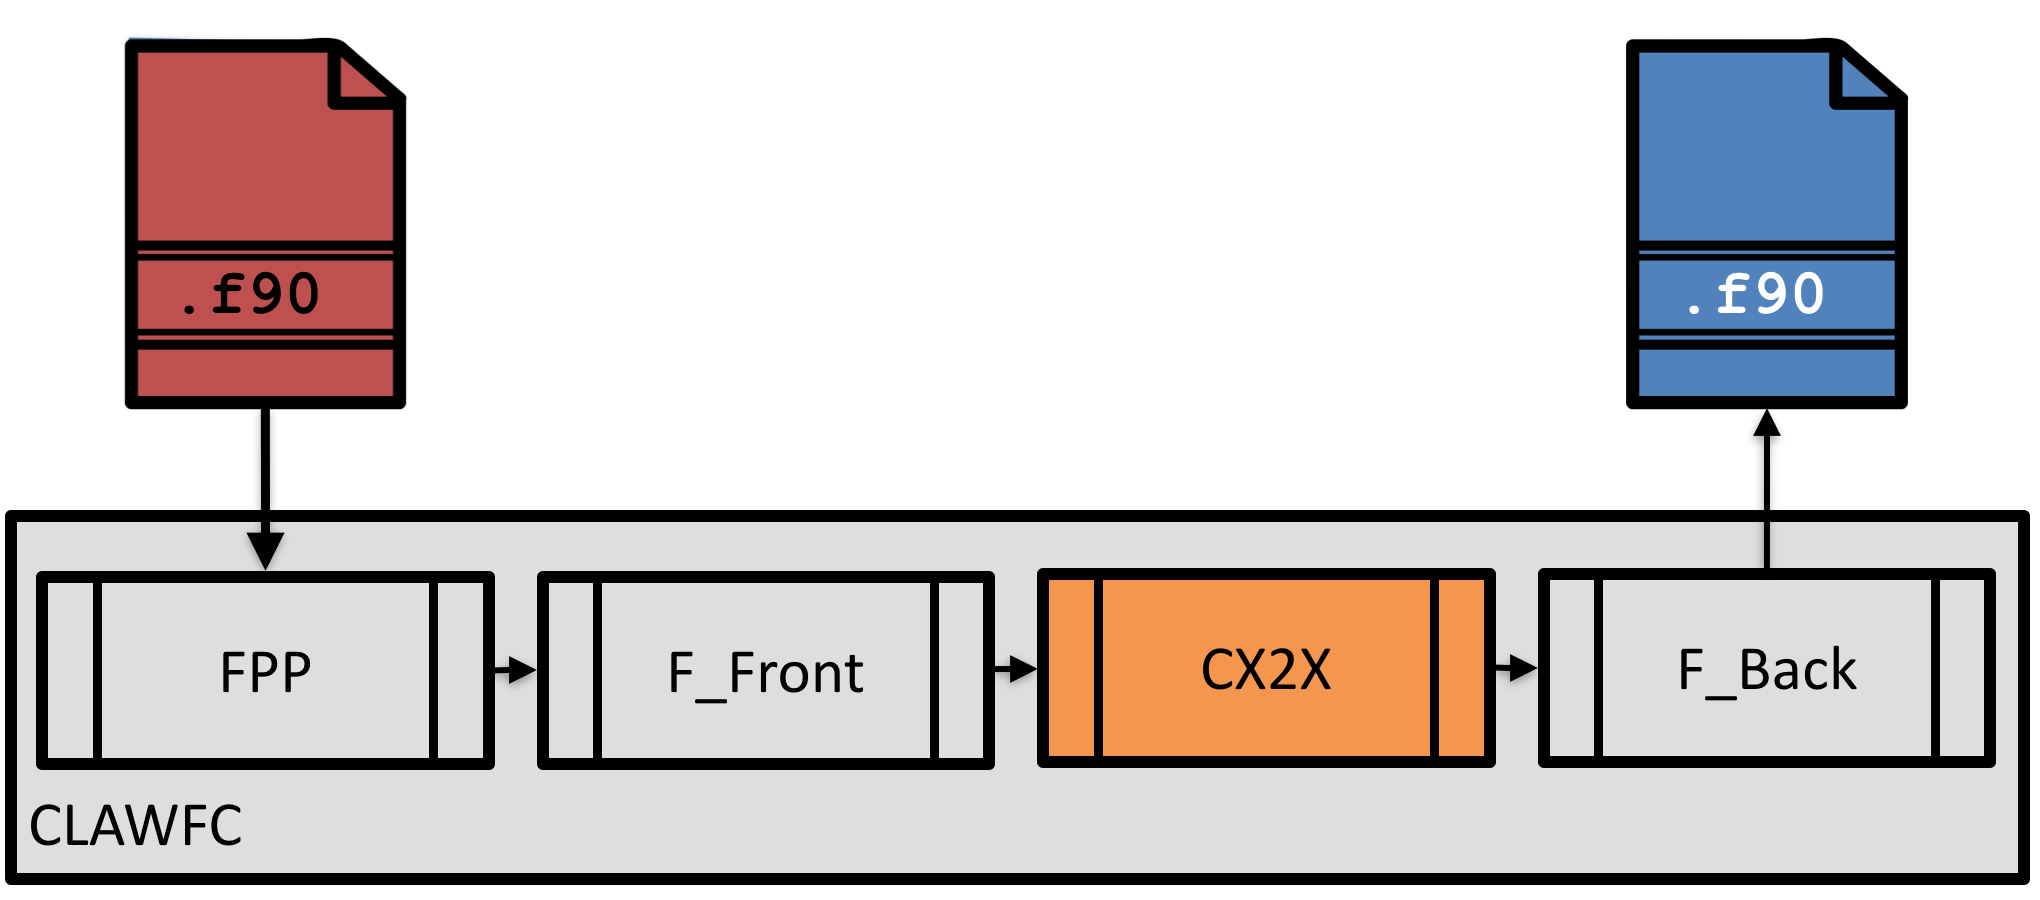
\includegraphics[
    width=0.8\textwidth
  ]{resources/clawfc_global_workflow.png} \\
  \caption{CLAW FORTRAN Compiler main workflow.}
  \label{fig:clawfc_main_workflow}
\end{figure}

\section{CLAW \xcodeml to \xcodeml translator}
The \xcodeml to \xcodeml translator is the intelligence of the \clawfcomp. It
understands the CLAW directive language and apply the corresponding
transformation to the \xcodeml \gls{ast}.

\begin{figure}[!ht]
  \centering
  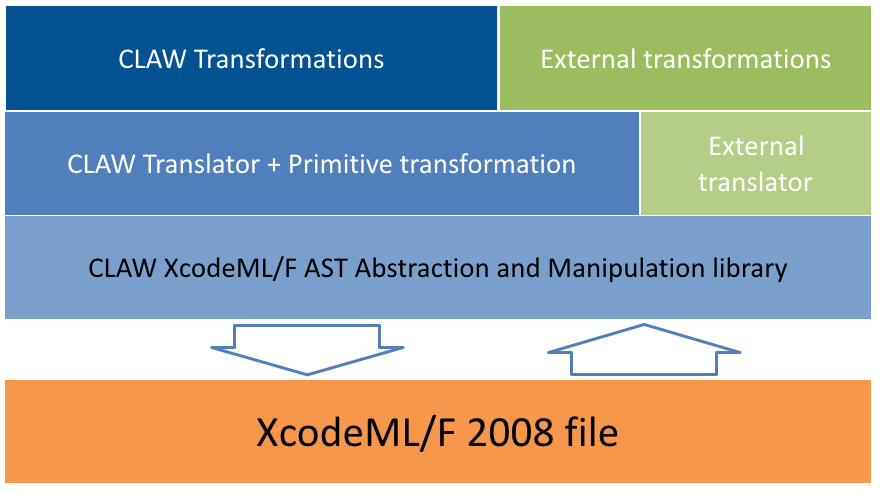
\includegraphics[width=0.8\textwidth]{resources/cx2x_stack.png} \\
  \caption{CLAW \xcodeml to \xcodeml library stack.}
  \label{fig:cx2x_stack}
\end{figure}

Figure \ref{fig:cx2x_stack} shows the stack of libraries used in the the CLAW
\xcodeml to \xcodeml translator. The two first layers from the bottom are
explained in more details in chapter \ref{chapter:astmanip}. The three last
layers are explained in chapter \ref{chapter:transformation}.
